\documentclass[conference]{IEEEtran}
\IEEEoverridecommandlockouts
% The preceding line is only needed to identify funding in the first footnote. If that is unneeded, please comment it out.
\usepackage{cite}
%\usepackage{natbib}
\usepackage{amsmath,amssymb,amsfonts}
\usepackage{algorithmic}
\usepackage{graphicx}
\usepackage{textcomp}
\usepackage{xcolor}
\usepackage{hyperref}
\usepackage{dblfloatfix} 
\usepackage{afterpage}
\usepackage{placeins}
\usepackage{comment}
\usepackage{caption}
\usepackage{tabto}
\usepackage[utf8]{inputenc}
\usepackage{tabularx}
\usepackage{float}
\usepackage{siunitx}
\usepackage{dcolumn}

\renewcommand\tabularxcolumn[1]{m{#1}}
\hypersetup{
    colorlinks=false,
    linkcolor=blue,
    filecolor=magenta,      
    urlcolor=cyan,
}
\def\BibTeX{{\rm B\kern-.05em{\sc i\kern-.025em b}\kern-.08em
    T\kern-.1667em\lower.7ex\hbox{E}\kern-.125emX}}

\graphicspath{Images/}




\begin{document}

\title{Cotton Care: Harnessing Transfer Learning for Real-Time Health Assessment with Mobile Devices\\}

\makeatletter
\newcommand{\linebreakand}{%
  \end{@IEEEauthorhalign}
  \hfill\mbox{}\par
  \mbox{}\hfill\begin{@IEEEauthorhalign}
}
\makeatother

\author{\IEEEauthorblockN{1\textsuperscript{st} Emerson A. de Lemmus}
\IEEEauthorblockA{\textit{Bioinformatics Group} \\
\textit{Cell Signaling Technology}\\
Boston, United States \\  
\href{https://orcid.org/0000-0001-8579-9453}{ORCID: 0000-0001-8579-9453}
}
\and
\IEEEauthorblockN{2\textsuperscript{nd} Brendan P. McAntosh}
\IEEEauthorblockA{\textit{Department of Computer Science} \\
\textit{Sam Houston State University}\\
Huntsville, United States \\ 
\href{https://orcid.org/0009-0008-7520-7432}{ORCID: 0009-0008-7520-7432}
}
\and
\IEEEauthorblockN{3\textsuperscript{rd} ABM Rezbaul Islam Ph.D.}
\IEEEauthorblockA{\textit{Department of Computer Science} \\
\textit{Sam Houston State University}\\
Huntsville, United States \\ 
\href{https://orcid.org/0000-0003-2610-7343}{ORCID: 0000-0003-2610-7343}
}
}



\maketitle

\begin{abstract}
Cotton frequently experiences substantial yield reduction due to disease afflictions. This paper introduces a proof-of-concept mobile application that employs transfer learning with pre-trained MobileNetV3 and NASNetMobile models to detect cotton plant diseases. The system addresses a four-class problem, identifying the health status of cotton plants or leaves. Using TensorFlow, these models are refined with publicly available data and deployed on an iOS app. This study also provides a performance assessment of both models, previously unexplored in this specific context. The methodology, showcasing significant potential for real-world implementations, recorded overall accuracies of 97.7\% for NASNetMobile and 96.7\% for MobileNetV3.
\end{abstract}

\begin{IEEEkeywords}
 Cotton Disease, Transfer Learning, MobileNetV3, NASNetMobile, Real-time detection, Mobile Application
\end{IEEEkeywords}

\section{Introduction}
According to the USDA's National Agriculture Statistics Service (NASS), Texas produced 6.32 million 480-pound bales of cotton in 2019, making it the top cotton-producing state in the country, accounting for approximately 33\% of the nation's total cotton production \cite{ USDA-NASS}. However, cotton is susceptible to various diseases, with 80-90\% of them, such as fungi and foliar leaf spots, manifesting on the cotton leaves \cite{Gulhane-Gurjar}. There is a demand for an accurate, affordable machine vision system to enable disease detection, which is crucial for optimal cotton growth and yield. Manual disease identification is time-consuming and labor-intensive; automating the process with modern avenues can enhance work efficiency and provide clear disease verification for agricultural experts.

The deep learning (DL) revolution has significantly impacted the AI industry in recent years. Since its 2012 victory over traditional machine learning algorithms in the ImageNet Large Scale Visual Recognition Challenge (ILSVRC), DL has become the leading solution for object recognition \cite{Ashqar-Naser}\cite{Gehlot-Saini}. Convolutional Neural Networks (CNNs) excel in object identification and image classification \cite{Sarangdhar-Pawar}.

Transfer learning, a popular approach in DL, leverages pre-trained CNNs for computer vision tasks instead of building a model from scratch \cite{Brownlee}. This technique reuses learned knowledge from one task for another, effectively addressing computational resource limitations in various applications, including computer vision, natural language processing, and speech recognition. 

With the increasing capability of edge devices, deploying computer vision models offers an accessible and practical approach to gathering real-world data insights. This study utilizes transfer learning to deliver plant health information via a mobile application, leveraging its proven efficacy in crop disease detection \cite{Disease Detection} \cite{Disease Diagnosing}. To increase the depth of our study, we leverage two state-of-the-art Google models -- MobileNetV3 (2019) and NASNetMobile (2018) \cite{WandB} -- created and optimised for mobile/edge devices. We employ a publicly available dataset \cite{Kaggle} which contains images and labels for healthy and diseased cotton leaves and plants. TensorFlow Lite is used to deploy models on mobile devices, simplifying the implementation of transfer learning.


\section{RELATED WORKS}

Numerous studies demonstrate the effectiveness of deep learning (DL) in plant disease detection and classification. For instance, Singh et al. \cite{Singh-etal} and Mohanty et al. \cite{Mohanty-etal} achieved detection accuracies of 96.9\% and 98.3\% for rice and cassava diseases, respectively. In cotton disease detection, both Bhoi \cite{Bhoi} and Dey et al.\cite{Dey-etal} utilized DL models, yielding accuracies above 90\%. Additionally, transfer learning has proven successful in disease detection, with Kazemi et al\cite{Kazemi-etal} and Sharma et al.\cite{Sharma-etal} achieving over 97\% accuracy for tomato and potato diseases, respectively. Mobile applications have also been effectively implemented. For instance, Siddique et al.\cite{Siddique-etal} and Uddin et al.\cite{Uddin-etal} developed mobile apps for wheat and mango disease detection using transfer learning, both achieving over 90\% accuracy. These studies underscore the utility of deep learning, transfer learning, and mobile applications in accessible, practical disease detection for agriculture.

\section{Methodology}

This study aims to demonstrate an accessible, efficient, and real-time mobile application for cotton disease detection, utilizing transfer learning. The app uses a mobile phone camera to provide instantaneous health classification of cotton plants or leaves, functioning even in areas with limited internet connectivity. In contrast to manual disease detection methods, which can be labor-intensive, expensive, and slow, a real-time mobile application can provide immediate classification. Importantly, we deploy MobileNetV3-Large and NASNetMobile, two previously unused computer vision models in the cotton disease domain space. This methodology also offers a performance baseline for cotton disease studies using future iterations of MobileNet and NASNet architectures. 


\subsection{Transfer Learning}

Transfer learning, leverages a pre-trained model—often trained on a large dataset like ImageNet—to fine-tune the learning process for a specific task \cite{Shu}. This approach capitalizes on the pre-trained model's generalized weights, facilitating swift prototyping of architectures while being cost-effective. For instance, training a model from scratch on ImageNet, a 14-million-image dataset \cite{Reynolds}, is prohibitively expensive for most researchers. In 2017, the cost for each training iteration was estimated at \$1,112.64, excluding upfront hardware costs \cite{genuineimpact}.

Depicted in \emph{Fig. \ref{Transfer Learning}}, transfer learning employs a pre-trained model, freezing most layers to preserve its weights, or knowledge, from training on millions of images. These frozen layers are beneficial due to their learned capacity to discern a variety of image features. However, for the recognition of new targets like diseased foliage, fine-tuning the model's unfrozen layers is crucial.

\begin{figure}[h]
\centerline{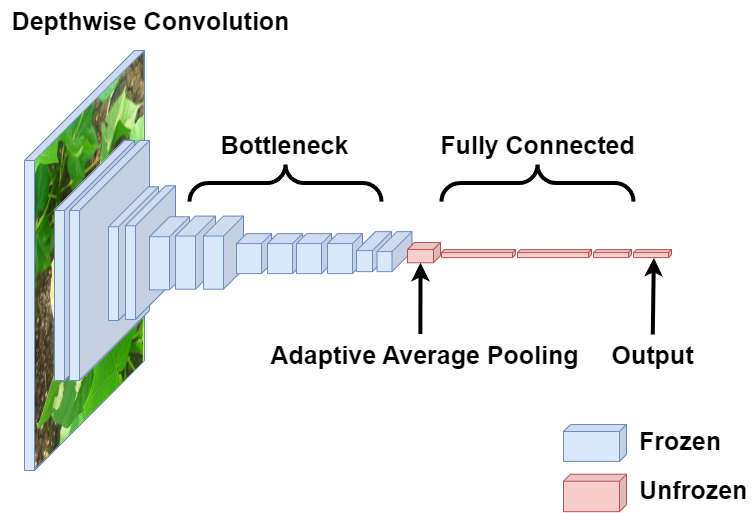
\includegraphics[height=6.5cm, width=1\linewidth]{Images/MobileNetV3_layers.drawio.png}}
\caption{Visualisation of a pre-trained model's architecture. The depicted architecture is inspired by MobileNetV3. Each block represents a model layer that is either frozen or unfrozen during transfer learning. It is common to preserve the core convolution layers found in the Depthwise and Bottleneck sections since they retain the ability to discern a wide range of image features. The pooling, fully connected, and output layers, also commonly found in many CNN models, must be retrained to identify new targets.}
\label{Transfer Learning}
\end{figure}

\subsection{Dataset}
We utilize a public dataset sourced from Kaggle \cite{Kaggle}. It contains 2,310 labeled images of cotton plants and leaves in the RGB colorspace. Images are classified into four categories: diseased cotton leaf, diseased cotton plant, fresh cotton leaf, and fresh cotton plant, as sampled in \emph{Fig. \ref{CottonImages}}. The split is 1764 training, 440 validation, and 106 testing images.  Both MobileNetV3 and NASNetMobile were trained with the same data with their training performance evaluated against the validation set and final overall accuracy against the testing set. 

\begin{figure}[h]
\centerline{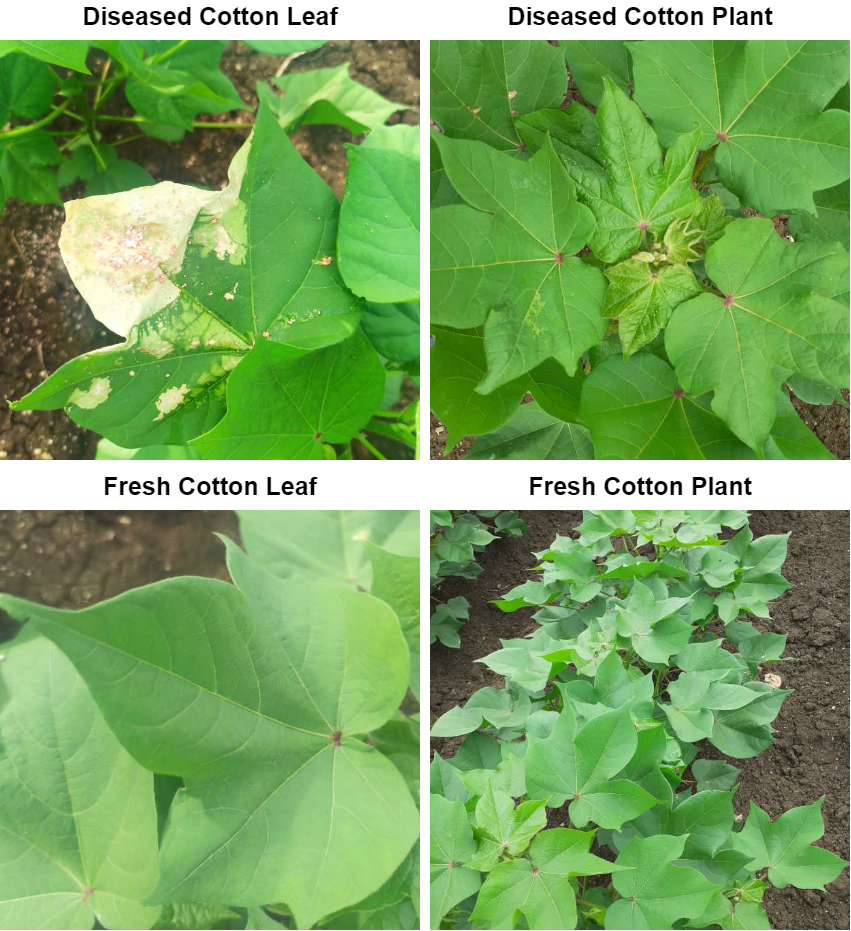
\includegraphics[height=8.5cm, width=.9\linewidth]{Images/cotton images.drawio.png}}
\caption{Sample images for each class featured in the dataset. Image credit: B. Janmejay.}
\label{CottonImages}
\end{figure}

\subsection{Data pre-processing}

For this study, we created a standard data pre-processing protocol for both models promoting learning equality across both models. It converts raw data into a trainable format and highlights key image features. The dataset was resized to 224 x 224 pixels to meet MobileNetV3 and NASNetMobile input requirements while preventing feature loss or compression artifacts. We augmented the data by creating modified copies of existing images, as shown in \emph{Fig. \ref{Augment}}, enhancing model generalization with transformations like rotation, flipping, shear, and zoom. \emph{Table \ref{table:DataAug}} details the augmentation parameters. Data augmentation expanded the dataset from 1763 to 8816 images. We split the augmented dataset 80/20 for training/validation and kept the original 106 test images.
 
\begin{figure*}[ht]
\centering
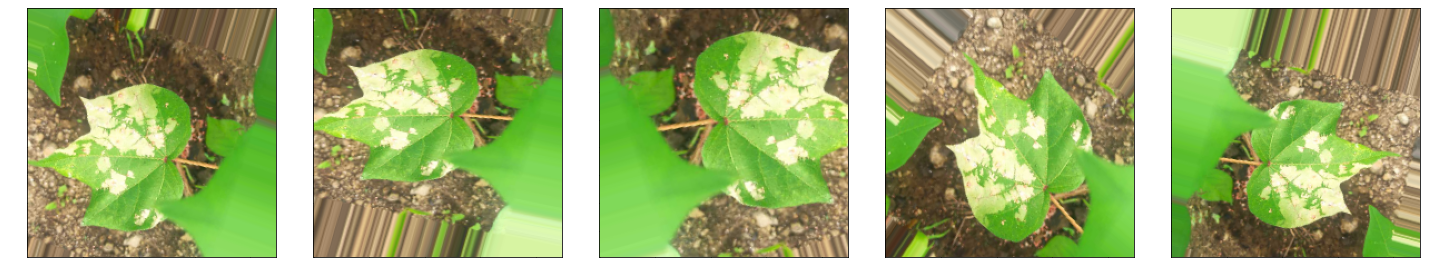
\includegraphics[height=3.2cm, width=1\linewidth]{Images/Data_Augmentation5.png}
\caption{Example of data augmentation techniques applied to an image: a raw image undergoes various transformations, such as rotation, scaling, flipping, and shearing, to increase the diversity of the training dataset and improve model generalization.}
\label{Augment}
\end{figure*}

\begin{table}[ht]
\centering
\caption{Data Augmentation Settings}
%\begin{tabular}{l|l}
\begin{tabularx}{1\columnwidth}{X|>{\centering\arraybackslash}X}
\hline
\textbf{Parameter} & \textbf{Value} \\
\hline
Rotation Range & 40 \\
Horizontal Flip & True \\
Width Shift & 0.2 \\
Height Shift & 0.2 \\
Shear Range & 0.2 \\
Zoom Range & 0.2 \\
Rescale & 1./255 \\
Validation Split & .20 \\
\hline
\end{tabularx}
\label{table:DataAug}
\end{table}


\subsection{Defining Convolutional Neural Networks}

Convolutional Neural Networks (CNNs), comprising sequential layers for processing input images, are a potent tool for image classification. The process begins with the first layer applying multiple convolution operations to the input image, generating a feature map matrix. This matrix undergoes dimension reduction through resizing as it progresses through the layers. The output from one layer serves as input to the subsequent layer, culminating in a fully connected layer that compacts all features into a vector for the final softmax layer, which in turn outputs the classifier labels and their associated probabilities.

Mathematically, the convolution operation performed in CNNs' initial layers can be expressed as:

\begin{equation}
Z(i,j) = (I * K)(i,j) = \sum_m \sum_n I(m,n) K(i-m,j-n)
\end{equation}

Here, $I$ is the input image, $K$ the filter kernel, and $Z(i,j)$ the output feature map matrix. The filter is applied to each element of the input image, with the resultant values summed to form each output matrix element.

Each layer's output is computed via:

\begin{equation}
A^{(l)} = g(Z^{(l)}) = g(W^{(l)}A^{(l-1)} + b^{(l)})
\end{equation}

In this equation, $W^{(l)}$ and $b^{(l)}$ denote the weights and biases of the $l$-th layer respectively, $A^{(l-1)}$ is the input feature map, $g$ represents the activation function, and $Z^{(l)}$ is the weighted sum of input features.

The final softmax layer computes classifier labels as follows:

\begin{equation}
P(y=j|x) = \frac{e^{z_j}}{\sum_{k=1}^K e^{z_k}}
\end{equation}

Here, $P(y=j|x)$ is the probability of classifying the image as label $j$, $z_j$ refers to the weighted sum of features for label $j$, and $K$ is the total number of labels \cite{Smeda}.


\subsection{MobileNetV3}

We selected MobileNetV3-Large, a state-of-the-art mobile CNN launched by Google in Q2 2019 for mobile and embedded vision applications \cite{Howard-Sandler}. The model uses depth-wise separable convolutions, reducing computations significantly \cite{Yanhui}. As per paperswithcode, the large model version, comprising 17 blocks, was chosen for its larger trainable parameters, accuracy, and similarity with NASNetMobile in parameters, FLOPS, and file size \cite{paperswithcode}. This architecture is suitable for deployment in resource-constrained devices \cite{Howard-Zhu}. Its default parameters are summarized in  \emph{Table \ref{table:MobileNetV3}}.


%and \emph{Table \ref{table:MobileNetV3-Architecture}}  and architecture

\begin{table}[ht]
\centering
\caption{MobileNetV3 - Parameters}
%\begin{tabular}{l|l}
\begin{tabularx}{1\columnwidth}{X|>{\centering\arraybackslash}X}
\hline
\textbf{Parameter} & \textbf{Value} \\
\hline
Trainable Parameters & 5 Million \\
FLOPS & 225 Million \\
File Size & 21.11 MB \\
Training Data & ImageNet \\
Training Resources & 8x NVIDIA V100 GPUs \\
\hline
\end{tabularx}
\label{table:MobileNetV3}
\end{table}

%\begin{table}[ht]
%\centering
%\caption{MobileNetV3 - Architecture}
%\begin{tabularx}{\columnwidth}{>{\centering\arraybackslash}X}
%\hline
%\begin{tabular}{c}
%1x1 Convolution \\
%Batch Normalization \\
%Convolution \\
%Dense Connections \\
%Depthwise Separable Convolution \\
%Dropout \\
%Global Average Pooling \\
%Hard Swish \\
%Inverted Residual Block \\
%Residual Connection \\
%ReLU \\
%Softmax \\
%Squeeze-and-Excitation Block \\
%\end{tabular} \\
%\hline
%\end{tabularx}
%\label{table:MobileNetV3-Architecture}
%\end{table}



\subsection{NASNetMobile}
The second model selected is NASNetMobile an advanced mobile CNN introduced by Google in 2018. NASNetMobile uses a neural architecture search (NAS) algorithm developed by Google Brain for the 2018 ImageNet Competition, which uses reinforcement learning to explore a large space of possible architectures and identifying the ones that perform best for a given task. The default architecture of NASNetMobile consists of 13 blocks and is based on a series of "normal" and "reduction" cells, with each cell performing a set of operations, including convolution, batch normalization, and activation. The output of each block is computed as:

\begin{equation}
H_{l,k} = F_{l,k}(H_{l-1,1},H_{l-1,2},...,H_{l-1,n})
\end{equation}

where $F_{l,k}$ is the function applied by the $k$-th block in the $l$-th cell, $H_{l-1,1},H_{l-1,2},...,H_{l-1,n}$ are the inputs to the $k$-th block from the previous cell, and $H_{l,k}$ is the output of the $k$-th block in the $l$-th cell. The final output of the NASNetMobile architecture is a softmax layer, which computes the probabilities of each class label given the input image.

NASNetMobile has been designed to be smaller and more efficient, suitable for use on mobile devices or other situations where computational resources are limited. The NAS algorithm allows for the automatic design of highly efficient and accurate models, saving time and resources compared to manual architecture design. \emph{Table \ref{table:NASNetMobile}} summarizes default NASNetMobile parameters concisely \cite{paperswithcodenas}. % \emph{Table \ref{table:NASNetMobile-Architecture}} 

\begin{table}[ht]
\centering
\caption{NASNetMobile - Parameters}
%\begin{tabular}{l|l}
\begin{tabularx}{1\columnwidth}{X|>{\centering\arraybackslash}X}
\hline
\textbf{Parameter} & \textbf{Value} \\
\hline
Trainable Parameters & 4 Million \\
FLOPS & 325 Million \\
File Size & 16.92 MB \\
Training Data & ImageNet \\
Training Resources & 8x NVIDIA V100 GPUs \\
\hline
\end{tabularx}
\label{table:NASNetMobile}
\end{table}

% \begin{table}[ht]
% \centering
% \caption{NASNetMobile - Architecture}
% \begin{tabularx}{\columnwidth}{>{\centering\arraybackslash}X}
% \hline
% \begin{tabular}{c}
% 1x1 Convolution \\
% Batch Normalization \\
% Convolution \\
% Depthwise Separable Convolution \\
% Dropout \\
% Global Average Pooling \\
% Inverted Residual Block \\
% Residual Connection \\
% ReLU \\
% Max Pooling \\
% Softmax \\
% Squeeze-and-Excitation Block \\
% \end{tabular} \\
% \hline
% \end{tabularx}
% \label{table:NASNetMobile-Architecture}
% \end{table}

%\begin{table}[ht]
%\centering
%\caption{NASNetMobile - Architecture}
%\begin{tabular}{l}
%\hline
%1x1 Convolution \\
%Batch Normalization \\
%Convolution \\
%Depthwise Separable Convolution \\
%Dropout \\
%Global Average Pooling \\
%Inverted Residual Block \\
%Residual Connection \\
%ReLU \\
%Max Pooling \\
%Softmax \\
%Squeeze-and-Excitation Block \\
%\hline
%\end{tabular}
%\label{table:NASNetMobile-Architecture}
%\end{table}



\section{Experimental Results}

Despite a brief 20-epoch training phase, Google Colab's free environment constrained the epoch count due to slower processing speed compared to local hardware. \emph{Table \ref{table:MNParam}} and \emph{Table \ref{table:NNMParam}} detail the training hyperparameters for each model. Performance evaluation of both models relied on metrics such as accuracy, recall, precision, and F1-score. \emph{Table \ref{table:MNCM}} and \emph{Table \ref{table:MNPerformance}}  present the confusion matrix and performance metrics for MobileNetV3, while \emph{Table \ref{table:NNMCM}}, and \emph{Table \ref{table:NNMPerformance}} detail the same for NASNetMobile.  

\begin{table}[htbp]
    \centering
    \caption{MobileNetV3 - Hyperparameters}
    \begin{tabularx}{1\columnwidth}{X|>{\centering\arraybackslash}X}
    \hline
    \multicolumn{1}{c|}{\textbf{Parameter}} & \multicolumn{1}{c}{\textbf{Value}} \\
    \hline
    Learning Rate & 0.064 \\
    Training Steps & 20 \\
    LR Gamma & 0.973 \\
    Momentum & 0.9 \\
    Batch Size & 128 \\
    LR Step Size & 2 \\
    Random Erase & 0.2 \\
    Weight Decay & 0.00001 \\
    \hline
    \end{tabularx}
    \label{table:MNParam}
\end{table}

\begin{table}[htbp]
    \centering
    \caption{NASNetMobile - Hyperparameters}
    \begin{tabularx}{1\columnwidth}{X|>{\centering\arraybackslash}X}
    \hline
    \multicolumn{1}{c|}{\textbf{Parameter}} & \multicolumn{1}{c}{\textbf{Value}} \\
    \hline
    Learning Rate & 0.1 \\
    Training Steps & 20 \\
    LR Gamma & 0.1 \\
    Momentum & 0.9 \\
    Batch Size & 32 \\
    LR Step Size & 30 \\
    Weight Decay & 0.0001 \\
    \hline
    \end{tabularx}
    \label{table:NNMParam}
\end{table}

\subsection{Results -  MobileNetV3}

According to TensorFlow metrics, after 20 training steps, the training and validation loss stood at 72.90\% and 75.92\%, respectively, with best validation and training accuracies at 98.66\% and 99.29\%. This underscores the model's effectiveness in correctly classifying cotton foliage into four categories. As shown in \emph{Fig. \ref{MNStats}}, the relationship between training and validation loss can be complex. Overfitting occurs when validation loss significantly surpasses training loss, and underfitting when training loss plateaus or drops without a corresponding decrease in validation loss. Initially, MobileNetV3 exhibited unstable loss metrics, but both losses eventually reached a semi-stable point with a minimal gap. Training and validation accuracies indicated a good fit, initially showing high bias before converging around training step 7.5.

\begin{figure}[h]
\centerline{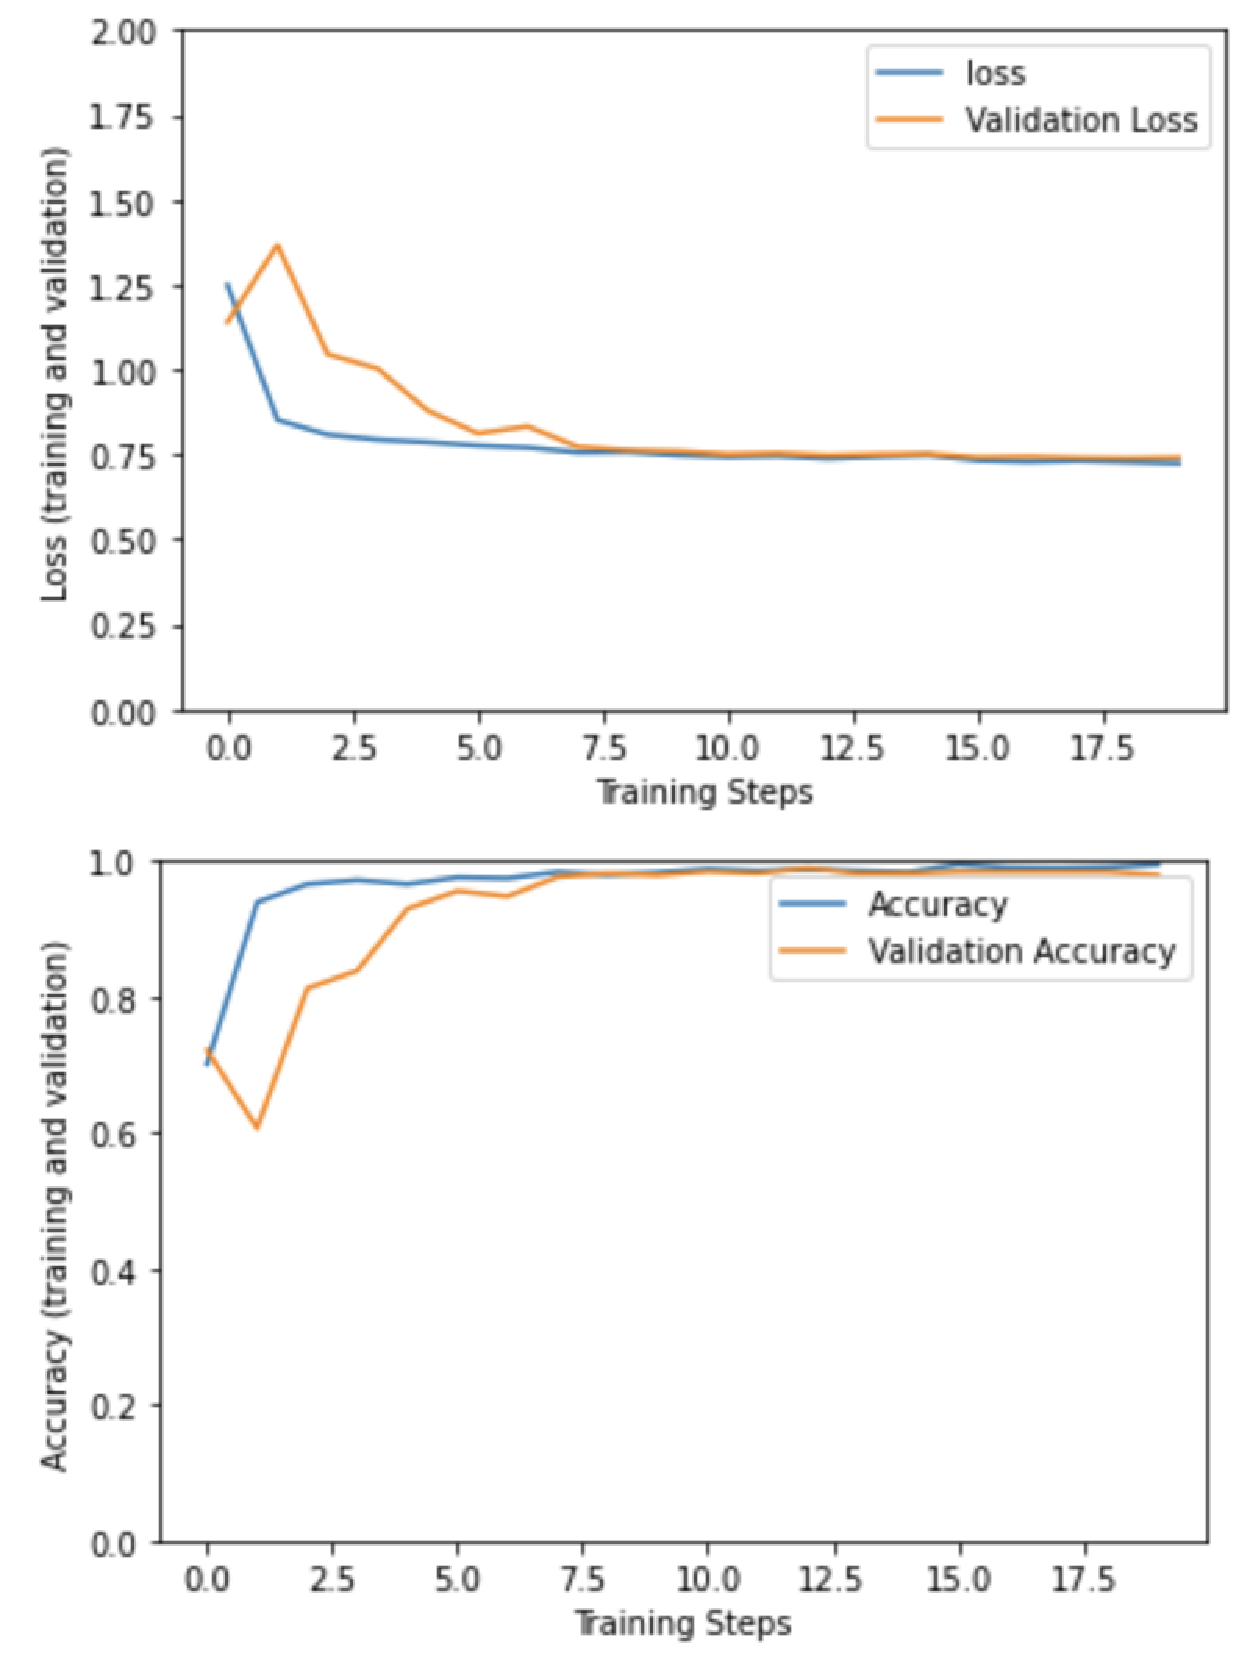
\includegraphics[height=10cm, width = .9\linewidth]{Images/Screen_Shot_2021-05-04_at_5.27.06_PM.pdf}}
\caption{MobileNetV3 training performance over 20 epochs. \centering{\newline Top: Plots training and validation loss against epochs. \newline Bottom: Plots accuracy and validation accuracy against epochs.}}
\label{MNStats}
\end{figure}

To evaluate model accuracy and robustness, we isolated 106 test images from the training process, using them as diverse, unseen data for performance assessment. This test phase gauges the model's generalization ability, essential for real-world applications. The test phase performances are presented in a confusion matrix in \emph{Table \ref{table:MNCM}}.

\begin{table}[htbp]
    \centering
    \caption{MobileNetV3 - Confusion Matrix}
    \label{table:MNCM}
    \begin{tabularx}{0.49\textwidth }{ 
        >{\centering\arraybackslash}X 
        >{\centering\arraybackslash}X 
        >{\centering\arraybackslash}X 
        >{\centering\arraybackslash}X 
        >{\centering\arraybackslash}X
        }
    \hline
    \textbf{Class (images)} & \textbf{Fresh Leaf} & \textbf{Fresh Plant} & \textbf{Diseased Leaf} & \textbf{Diseased Plant} \\
    \hline 
    Fresh Leaf (26) & 24 & 0 & 2 & 0 \\
    Fresh Plant (27) & 0 & 22 & 0 & 5 \\
    Diseased Leaf (25) & 0 & 0 & 24 & 1 \\ 
    Diseased Plant (28) & 0 & 0 & 0 & 28 \\
    \hline
    \end{tabularx} 
\end{table}

The overall accuracy of the proposed model is given by equation \ref{eq:oa}:
\begin{equation}
Overall Accuracy = \frac{TP + TN}{TP+TN+FP+FN}
\label{eq:oa}
\end{equation}

where TP represents true positive, TN represents true negative, FP represents false positive, and FN represents false negative.\newline


Using transfer learning, our MobileNetV3 model achieved high accuracy rates for each label; the overall accuracy of the model was 96.7\% as calculated using equation \ref{eq:oa}. These results demonstrate the effectiveness of our model in accurately identifying and classifying the health status of cotton foliage. Notably, the model performed the lowest when classifying fresh plants. The reason for this inconsistency may be explained by the visual similarity between a fresh cotton plant and a diseased cotton plant as demonstrated in \emph{Fig. \ref{Diseased_Fresh_Plant}}, it can be challenging to differentiate even with human vision.

\begin{table}[htbp]
    \centering
    \caption{MobileNetV3 - Test Performance Metrics}
    \label{table:MNPerformance}
    \begin{tabularx}{0.49\textwidth }{ 
        >{\centering\arraybackslash}X 
        >{\centering\arraybackslash}X 
        >{\centering\arraybackslash}X 
        >{\centering\arraybackslash}X 
        >{\centering\arraybackslash}X
        >{\centering\arraybackslash}X
        }
    \hline
    \textbf{Class} & \textbf{Recall} & \textbf{Precision} & \textbf{F1-Score} & \textbf{Test Accuracy} \\
    \hline 
    Fresh Leaf & 0.923 & 1.000 & 0.960 & 97.5\% \\
    Fresh Plant & 1.000 & 0.815 & 0.898 & 94.8\% \\
    Diseased Leaf & 0.960 & 0.960 & 0.960 & 97.5\% \\
    Diseased Plant & 1.000 & 1.000 & 1.000 & 100\% \\
    \hline
    \end{tabularx} 
\end{table}

\begin{figure}[h]
\centerline{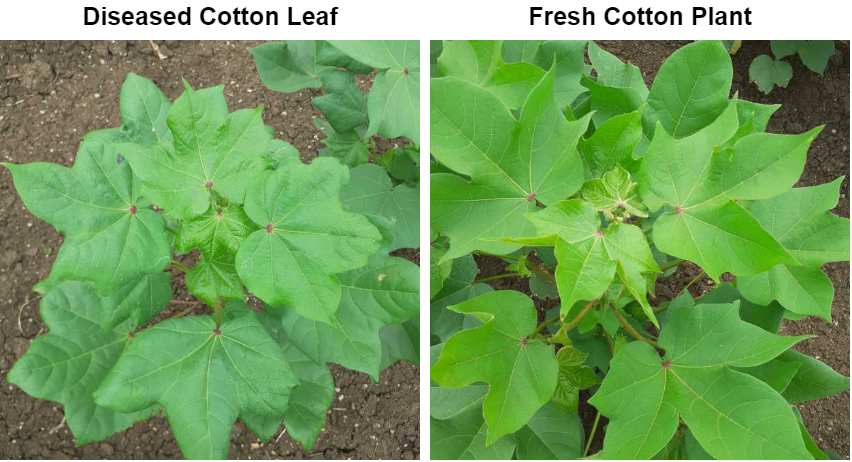
\includegraphics[height=5cm, width=1\linewidth]{Images/Disease_FreshComparison.drawio.png}}
\caption{Displayed are two randomly selected images from the Kaggle dataset, illustrating the occasional visual similarity between different classes. It is difficult to distinguish the difference - even with human vision. This attribute contributes to the lower F1-Score (0.898) and Accuracy (94\%) for the Fresh Plant class when using MobileNetV3 for inference. Image credit: B. Janmejay.}
\label{Diseased_Fresh_Plant}
\end{figure}


\subsection{Results - NASNetMobile}

A similar evaluation process was performed for NASNetMobile. Shown in \emph{Fig. \ref{NNMStats}} after a training iteration for 20 epochs, the resulting training loss and validation loss were observed to be 75.48\% and 77.41\%, respectively. The loss curves exhibit very stable training results compared to MobileNetV3. The best validation accuracy of 98.77\% and the best training accuracy was 99.83\%. Similarly, the training curves initially exhibit a smaller bias and then quickly converge at training step 2.5. Evaluation of both learning curves indicates NASNetMobile will outperform MobileNetV3 despite NASNetMobile being a year older and containing 1 million fewer parameters than MobileNetV3. The superior training performance may be attributed to the automated neural architecture search (NAS) algorithm. NAS automatically adapts optimal architecture, including hyperparameters, filter sizes, output channels, and convolution layer count, thereby ensuring tailored performance for the given dataset \cite{Yanhui}.

\begin{figure}[h]
\centerline{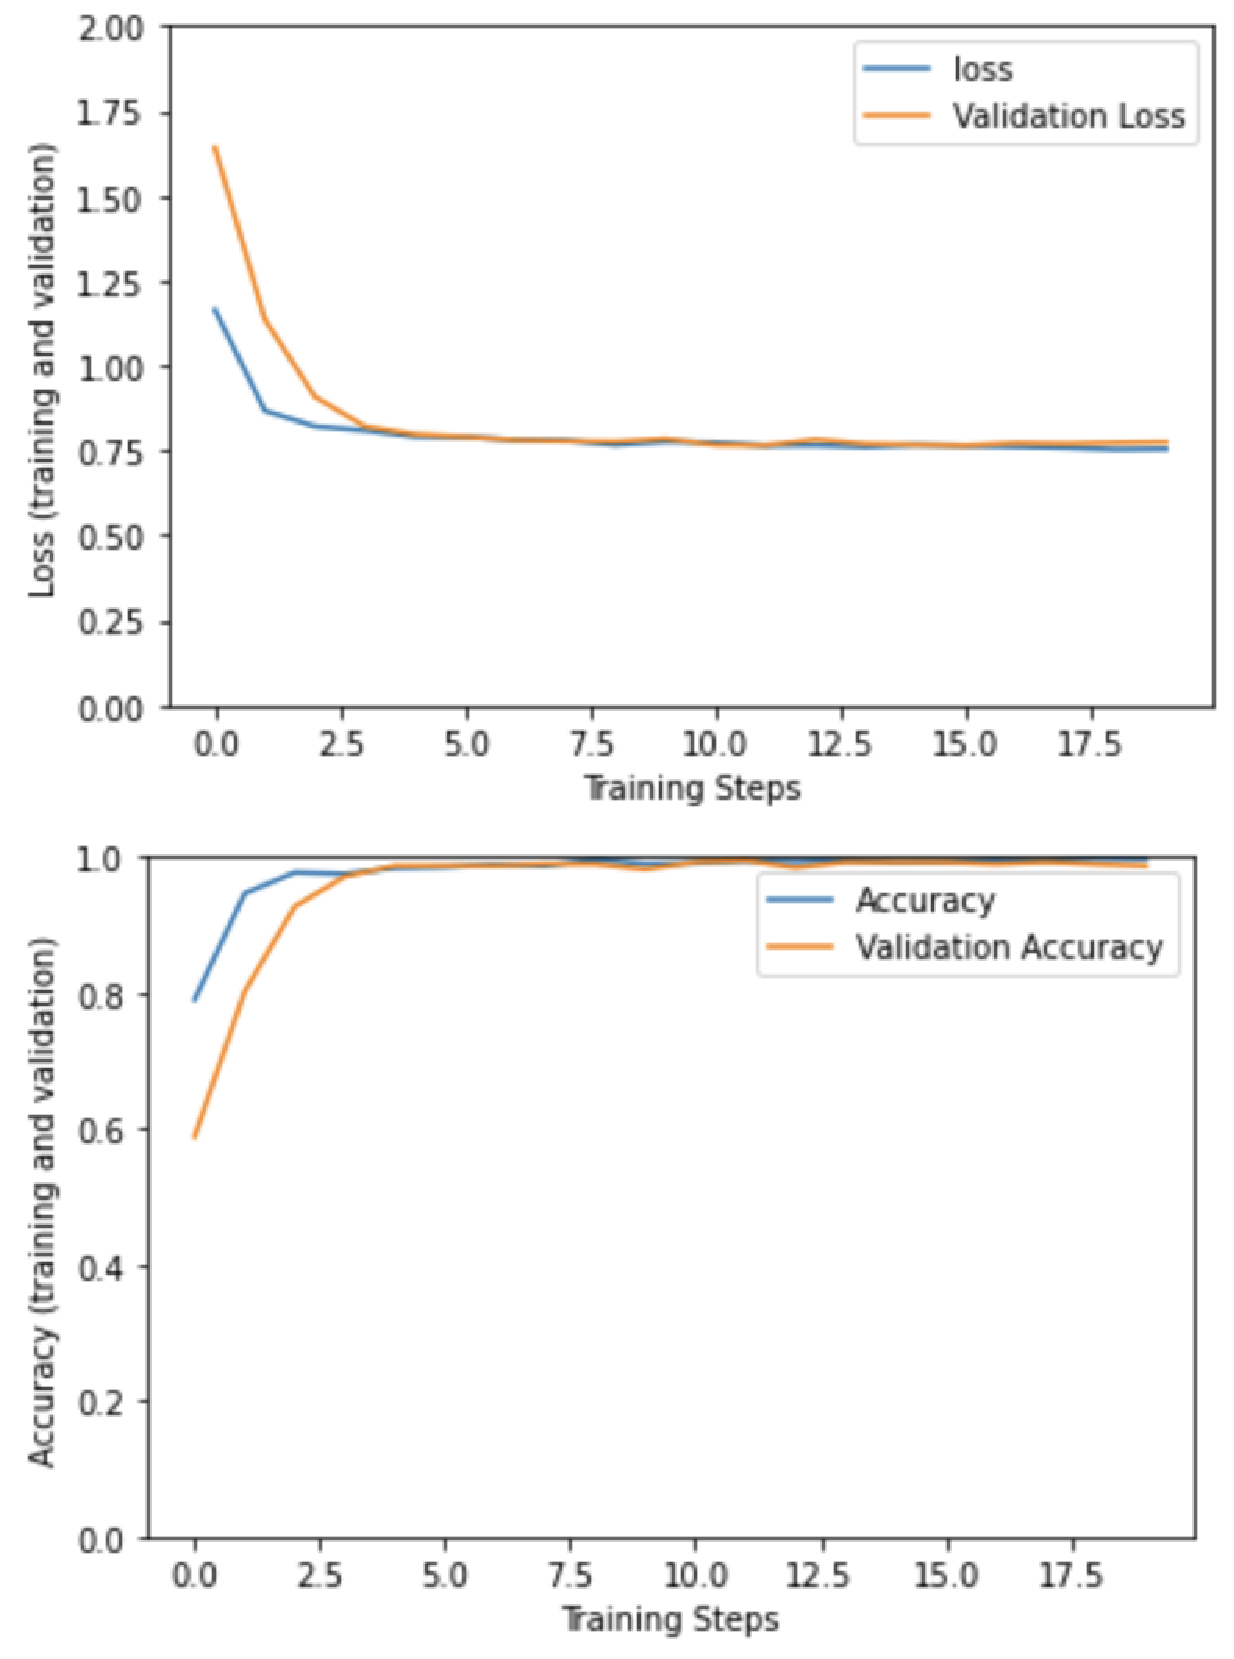
\includegraphics[height=10cm, width = .9\linewidth]{Images/Screen Shot 2021-05-10 at 4.36.35 PM.pdf}}
\caption{NASNetMobile training performance over 20 epochs. \centering{\newline Top: Plots of training and validation loss against epochs. \newline Bottom: Plots of accuracy and validation accuracy against epochs.}}
\label{NNMStats}
\end{figure}

The same 106 test images used for MobileNetV3 were also isolated to evaluate NASNetMobile's accuracy and robustness. It is imperative to note that high training metrics don't assure optimal test performance. NASNetMobile's confusion matrix is displayed in \emph{Table \ref{table:NNMCM}}.

\begin{table}[htbp]
    \centering
    \caption{NASNetMobile - Confusion Matrix}
    \label{table:NNMCM}
    \begin{tabularx}{0.49\textwidth }{ 
        >{\centering\arraybackslash}X 
        >{\centering\arraybackslash}X 
        >{\centering\arraybackslash}X 
        >{\centering\arraybackslash}X 
        >{\centering\arraybackslash}X
        }
    \hline
    \textbf{Class (images)} & \textbf{Fresh Leaf} & \textbf{Fresh Plant} & \textbf{Diseased Leaf} & \textbf{Diseased Plant} \\
    \hline 
    Fresh Leaf (26) & 26 & 0 & 0 & 0 \\
    Fresh Plant (27) & 1 & 25 & 0 & 1 \\
    Diseased Leaf (25) & 2 & 0 & 23 & 0 \\
    Diseased Plant (28) & 0 & 0 & 0 & 28 \\
    \hline
    \end{tabularx} 
\end{table}

Evaluating the NASNetMobile model during the test phase, delivered high accuracy for each label, achieving an overall accuracy of 97.7\%, outperforming MobileNetV3's 96.7\%. Despite being older and smaller, NASNetMobile outclassed MobileNetV3 in all categories, as demonstrated in \emph{Table \ref{table:NNMPerformance}}. Notably, it overcame MobileNetV3's classification challenge with Fresh Cotton Plants. 


\begin{table}[htbp]
    \centering
    \caption{NASNetMobile - Test Performance Metrics}
    \label{table:NNMPerformance}
    \begin{tabularx}{0.49\textwidth }{ 
        >{\centering\arraybackslash}X 
        >{\centering\arraybackslash}X 
        >{\centering\arraybackslash}X 
        >{\centering\arraybackslash}X 
        >{\centering\arraybackslash}X
        }
    \hline
    \textbf{Class} & \textbf{Recall} & \textbf{Precision} & \textbf{F1-Score} & \textbf{Test Accuracy} \\
    \hline 
    Fresh Leaf & 1.000 & 0.897 & 0.945 & 98.8\% \\
    Fresh Plant & 0.926 & 0.962 & 0.944 & 96.1\% \\
    Diseased Leaf & 0.920 & 0.920 & 0.920 & 97.7\% \\
    Diseased Plant & 1.000 & 1.000 & 1.000 & 100\% \\
    \hline
    \end{tabularx} 
\end{table}

\section{Mobile Application}

The mobile application, developed on the iOS platform using TensorFlow Lite, incorporates both MobileNetV3 and NASNetMobile for real-time classification, as shown in \emph{fig. \ref{DiseasedCottonLeaf}}. During the testing phase, all 106 test images were scanned using this application on an iPhone 12 Pro Max. The absence of an Android version, due to the lack of a comprehensive solution for model bundling and loading for both platforms, can be addressed in future iterations. The compact mobile application, with each model not exceeding 21.11 MB, provides a portable solution for cotton disease classification, presenting significant potential impact on the agricultural industry.

\begin{figure}[h]
\centerline{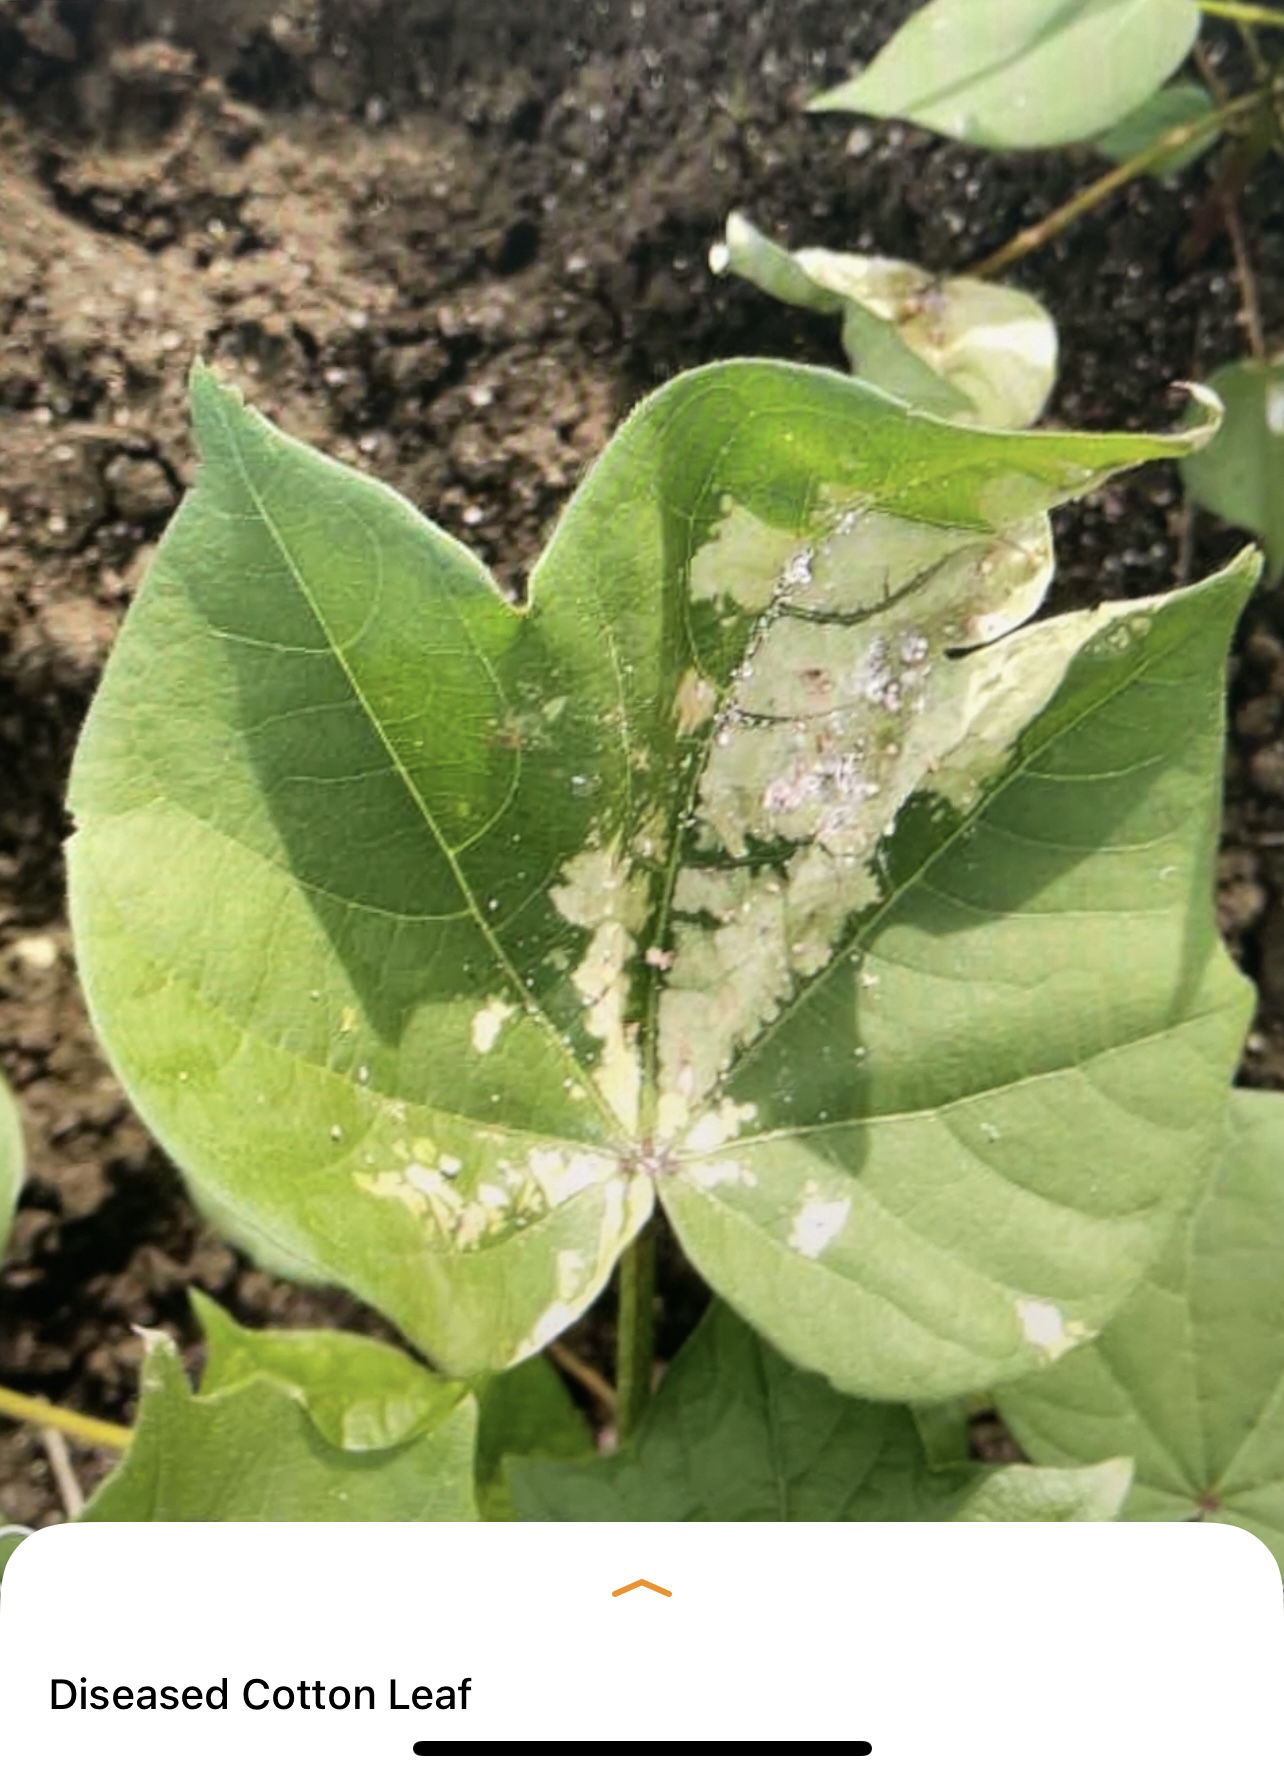
\includegraphics[height=11.5cm, width =.9\linewidth]{Images/Diseased Cotton Leaf.png}}
\caption{An iOS application demo classifying a diseased cotton leaf in real-time.}
\label{DiseasedCottonLeaf}
\end{figure}

\section{Future Developments}

\subsection{Dataset Expansion}

The Kaggle dataset used in this study, while sufficient for a proof-of-concept, lacks the comprehensive and robust nature necessary for a thorough disease detection system. Ideally, the dataset would incorporate specific disease labels for both foliar and root ailments, facilitating more nuanced classification beyond the binary healthy/diseased distinction. The dataset's limitations also extend to early disease lifecycle detection. The early-stage disease manifestation makes it difficult, even for human eyes, to differentiate between healthy/diseased classes. An improved and expanded dataset with expertly annotated labels could address these mentioned limitations and potentially stimulate new avenues of experimentation.

\subsection{Recommender System}

By expanding the dataset, possibly through merging distinct sources with specific disease labels, a compact recommender system could be implemented, suggesting potential remedies or disease treatments. This strategy, as exemplified by the PlantVillage Nuru system by Pennsylvania State University \cite{PlantVillage}, could particularly benefit underserved communities, delivering an offline, region-specific system demanding minimal updates in regions where cotton cultivation forms a substantial income source.

\subsection{Scalability}



\section{Conclusion}

This study highlights the simplicity and efficiency of transfer learning for training two advanced mobile-compatible models, NASNetMobile and MobileNetV3. Fine-tuning these models for cotton health classification yielded overall accuracies of 97.7\% and 96.7\% respectively, demonstrating NASNetMobile's superior performance, despite having fewer trainable parameters and being older. Notably, NASNetMobile excelled in identifying fresh cotton plants, a task challenging for MobileNetV3, likely due to NASNetMobile's self-updating architecture during training. The straightforward deployment of these models on an iOS application via TensorFlow Lite underscores the feasibility of this process, requiring only basic hardware and minimal upfront costs.

\section{Acknowledgment}

The authors extend their profound gratitude to the following individuals whose valuable insights, technical advice, and feedback significantly contributed to the realization of this research. 

We thank Dr. Hyuk Cho (Sam Houston State University) for his instrumental role in proposing the research topic, providing the initial dataset, and offering continuous insightful guidance. We thank Caitlyn T. Landrum and David C. Schmitt for providing technical contributions to the figures. We thank Stephen W. Smith for useful discussions.


%\bibliography{references}

    
\begin{thebibliography}{00}

\bibitem{USDA-NASS} National Agricultural Statistics Service, "Annual Cotton Review," [Online] Available: \href{https://www.nass.usda.gov/Statistics_by_State/Texas/Publications/Current_News_Release/2020_Rls/tx-cotton-review-2020.pdf}{nass.usda.gov}, 2019.

\bibitem{Gulhane-Gurjar} V. A. Gulhane and A. A. Gurjar, "Detection of Diseases on Cotton Leaves and Its Possible Diagnosis," \textit{International Journal of Image Processing (IJIP)}, vol. 5, no. 5, 2011.

\bibitem{Ashqar-Naser} Belal A.M. Ashqar, Samy S. Abu-Naser, "Image-Based Tomato Leaves Diseases Detection Using Deep Learning," International Journal of Academic Engineering Research (IJAER), Vol. 2, Issue 12, December 2018, pp. 10-16, ISSN: 2000-001X

\bibitem{Gehlot-Saini} Mamta Gehlot and Madan Lal Saini, "Analysis of Different CNN Architectures For Tomato Leaf Disease Classification," 5th IEEE International Conference on Recent Advances and Innovations in Engineering, ICRAIE 2020 (IEEE Record\#51050), 2020. 

\bibitem{Sarangdhar-Pawar} A. A. Sarangdhar and V. R. Pawar, "Machine learning regression technique for cotton leaf disease detection and controlling using IoT," in \textit{2017 International Conference of Electronics, Communications and Aerospace Technology (ICECA)}, 2017, vol. 2, pp. 449-454.

\bibitem{Brownlee} J. Brownlee, "A Gentle Introduction to Transfer Learning for Deep Learning," Machine Learning Mastery, December, 2017. [Online], Available: \href{https://machinelearningmastery.com/transfer-learning-for-deep-learning/#:~:text=Transfer\%20learning\%20is\%20a\%20machine,model\%20on\%20a\%20second\%20task.&text=Common\%20examples\%20of\%20transfer\%20learning,your\%20own\%20predictive\%20modeling\%20problems.}{machinelearningmastery.com}

\bibitem{Disease Detection} O. Kulkarni, "Crop Disease Detection Using Deep Learning," \textit{2018 Fourth International Conference on Computing Communication Control and Automation (ICCUBEA)}, Pune, India, 2018, pp. 1-4, doi: 10.1109/ICCUBEA.2018.8697390.

\bibitem{Disease Diagnosing} H. Park, E. JeeSook and S. Kim, "Crops Disease Diagnosing Using Image-Based Deep Learning Mechanism," \textit{2018 International Conference on Computing and Network Communications (CoCoNet)}, Astana, Kazakhstan, 2018, pp. 23-26, doi: 10.1109/CoCoNet.2018.8476914.

\bibitem{WandB} C. Lepelaars, "The Evolution Of Mobile CNN Architectures," \textit{WandB}, 8 November 2022, [Online], Available: \href{https://wandb.ai/carlolepelaars/mobile_architectures/reports/The-Evolution-Of-Mobile-CNN-Architectures--VmlldzoyMDQ0ODQ}{wandb.ai}

\bibitem{Kaggle} B. Janmejay, "Cotton Disease Dataset," \textit{Kaggle}, 24 September 2020, [Online] Available: \href{https://www.kaggle.com/janmejaybhoi/cotton-disease-dataset/notebooks}{kaggle.com}


\bibitem{Singh-etal} A. Singh, B. Ganapathysubramanian, S. Sarkar, and A. K. Singh, "Deep learning for plant stress phenotyping: Trends and future perspectives," \textit{Frontiers in Plant Science}, vol. 7, p. 1510, 2016.

\bibitem{Mohanty-etal} S. P. Mohanty, D. P. Hughes, and M. Salathé, "Using deep learning for image-based plant disease detection," \textit{Frontiers in Plant Science}, vol. 7, p. 1419, 2016.

\bibitem{Bhoi} J. M. Bhoi, "Identification of diseases in cotton leaves using machine learning," \textit{Research Square}, 2020.

\bibitem{Dey-etal} P. Dey, P. Roy, and S. Dey, "Automated classification of cotton leaf diseases using deep belief network," \textit{Computers and Electronics in Agriculture}, vol. 173, p. 105413, 2020.

\bibitem{Kazemi-etal} S. H. Kazemi, S. Mohsenzadeh, and A. Fooladgar, "A deep transfer learning approach for tomato diseases detection," \textit{Computers and Electronics in Agriculture}, vol. 162, pp. 706-713, 2019.

\bibitem{Sharma-etal} P. Sharma, A. K. Pandey, and M. Singh, "Potato disease classification using transfer learning approach," \textit{Agricultural Research}, vol. 10, no. 1, pp. 57-66, 2021.

\bibitem{Siddique-etal} A. B. Siddique, M. N. Akhtar, and M. Shafique, "Deep Learning Based Plant Disease Recognition using Mobile Devices," \textit{Procedia Computer Science}, vol. 171, pp. 1129-1136, 2020.

\bibitem{Uddin-etal} M. S. Uddin, M. A. H. Bhuiyan, M. R. Islam, and M. Z. Alom, "A deep learning based mobile application for mango disease detection," \textit{Computers and Electronics in Agriculture}, vol. 186, p. 106024, 2021.

\bibitem{Shu} M. Shu, "Deep Learning for image classification on very small datasets using transfer learning," Iowa State University, Summer 2019.

\bibitem{Reynolds} R. Reynolds, "New computer vision challenge wants to teach robots to see in 3D," \textit{NewScientist}, vol. 234, no. 3123, pp. 28-31, Apr. 2017, Available: \href{https://www.newscientist.com/article/2127131-new-computer-vision-challenge-wants-to-teach-robots-to-see-in-3d/}{NewScientist.com}.

\bibitem{genuineimpact} genuineimpact, "Cost to train AI system," genuineimpact, 2021. [Online]. Available: \href{https://i.redd.it/c9lyy4252qia1.png}{genuineimpact.com}.

\bibitem{Smeda} K. Smeda, "Understand the Architecture of CNN," \textit{Towards Data Science}, Oct. 2019. [Online]. Available: \href{https://towardsdatascience.com/understand-the-architecture-of-cnn-90a25e244c7}{Towards Data Science}.


\bibitem{Howard-Sandler} A. Howard, M. Sandler, et al., "Searching for MobileNetV3," in \textit{2019 IEEE/CVF International Conference on Computer Vision (ICCV)}, Seoul, Korea (South), 2019, pp. 1314-1324, doi: 10.1109/ICCV.2019.00140.

\bibitem{Yanhui} C. Yanhui, "From AlexNet to NASNet: A Brief History and Introduction of Convolutional Neural Networks," \textit{Towards Data Science}, 2021. [Online]. Available: \href{https://towardsdatascience.com/from-alexnet-to-NASNet-a-brief-history-and-introduction-of-convolutional-neural-networks-cf63bf3320e1}{towardsdatascience.com}

\bibitem{paperswithcode} paperswithcode, "MobileNet V3 Large", \textit{paperswithcode}, 2021. [Online] Available: \href{https://paperswithcode.com/lib/torchvision/mobilenet-v3}{paperswithcode.com}

\bibitem{Howard-Zhu} A. G. Howard, M. Zhu, B. Chen, D. Kalenichenko, W. Wang, T. Weyand, M. Andreetto, and H. Adam, "Mobilenets: Efficient convolutional neural networks for mobile vision applications," \textit{arXiv preprint} arXiv:1704.04861, 2017.

\bibitem{paperswithcodenas} paperswithcode, "NASNetMobile", \textit{paperswithcode}, 2021. [Online] Available: \href{https://paperswithcode.com/lib/torchvision/mnasnet-1-0}{paperswithcode.com}


\bibitem{PlantVillage} PlantVillage, "Solutions - Nuru", \textit{PlantVillage PSU}, 2020. [Online]. Available: \href{https://plantvillage.psu.edu/projects}{plantvillage.com}

%\bibitem{Shorten-Khosh} Shorten, C., Khoshgoftaar, T.M. ``A survey on Image Data Augmentation for Deep Learning''. J Big Data 6, 60 (2019). https://doi.org/10.1186/s40537-019-0197-0

%\bibitem{Gulhane-Gurjar} Mr. Viraj A. Gulhane and Dr. Ajay A. Gurjar, ``Detection of Diseases on Cotton Leaves and Its Possible Diagnosis``, International Journal of Image Processing (IJIP), vol. 5., issue: 5, 2011.

%\bibitem{Zoph-Vasudevan} Barret Zoph, Vijay Vasudevan et. al., ``Learning Transferable Architectures for Scalable Image Recognition'', Google Brain, April 2018.

%\bibitem{Simonyan-Zisserman} Karen Simonyan, Andrew Zisserman. ``Very Deep Convolutional Networks For Large-Scale Image Recognition'', Department of Engineering Science, University of Oxford. April 2015. 

%\bibitem{Neurohive} ``VGG16 - Convolutional Network for Classification and Detection''. November 2018. Available at \href{https://neurohive.io/en/popular-networks/vgg16/}{Neurohive.com}


%\bibitem{Progrev} ``How to Prevent Overfitting | Regularization''. Available at \href{https://programming-review.com/machine-learning/overfitting#cross-validation}{programming-review.com}

%\bibitem{Brownlee2} Jason Brownlee. ``How to use Learning Curves to Diagnose Machine Learning Model Performance''. Machine Learning Mastery. February 2019. Available at \href{https://machinelearningmastery.com/learning-curves-for-diagnosing-machine-learning-model-performance/}{machinelearningmastery.com}

%\bibitem{Stackexchange} ``Validation Accuracy vs Training Accuracy''. Available at \href{https://stats.stackexchange.com/questions/401696/validation-accuracy-vs-testing-accuracy}{stackexchange.com}


%\bibitem{Singh-et-al} Singh, A., Ganapathysubramanian, B., Sarkar, S., & Singh, A. K. (2016). Deep learning for plant stress phenotyping: Trends and future perspectives. Frontiers in plant science, 7, 1510.

%\bibitem{Mohanty-et-al} Mohanty, S. P., Hughes, D. P., & Salathé, M. (2016). Using deep learning for image-based plant disease detection. Frontiers in plant science, 7, 1419.

%\bibitem{Bhoi} Bhoi, J. M. (2020). Identification of diseases in cotton leaves using machine learning. Research Square.

%\bibitem{Dey-et-al} Dey, P., Roy, P., & Dey, S. (2020). Automated classification of cotton leaf diseases using deep belief network. Computers and Electronics in Agriculture, 173, 105413.

%\bibitem{Kazemi-et-al} Kazemi, S. H., Mohsenzadeh, S., & Fooladgar, A. (2019). A deep transfer learning approach for tomato diseases detection. Computers and Electronics in Agriculture, 162, 706-713.

%\bibitem{Sharma-et-al} Sharma, P., Pandey, A. K., & Singh, M. (2021). Potato disease classification using transfer learning approach. Agricultural Research, 10(1), 57-66.

%\bibitem{Siddique-et-al} Siddique, A. B., Akhtar, M. N., & Shafique, M. (2020). Deep Learning Based Plant Disease Recognition using Mobile Devices. Procedia Computer Science, 171, 1129-1136.

%\bibitem{Uddin-et-al} Uddin, M. S., Bhuiyan, M. A. H., Islam, M. R., & Alom, M. Z. (2021). A deep learning based mobile application for mango disease detection. Computers and Electronics in Agriculture, 186, 106024.

% \bibitem{m} M. Abd Elaziz, A. Dahou, N. A. Alsaleh, A. H. Elsheikh, A. I. Saba, and M. Ahmadein, "Boosting COVID-19 image classification using MobileNetV3 and aquila optimizer algorithm," \textit{Entropy}, vol. 23, no. 11, pp. 1383, 2021.




\end{thebibliography}






%\bibliographystyle{abbrv}
%\bibliography{references}


\end{document}
